\documentclass[11pt,a4paper]{article}
\usepackage{amssymb}
\usepackage{amsmath}
\usepackage{graphicx}
\usepackage{amscd}
\usepackage{vmargin}
\usepackage{mathrsfs,color,comment}
\usepackage{cases}
\usepackage{xfrac}
\usepackage{amsthm}
\usepackage{parskip}
\usepackage{mathtools}
\usepackage{xparse}
\usepackage{listings}
\usepackage{biblatex}
\usepackage{matlab-prettifier}
\usepackage{nicematrix}
\usepackage{bm}
\usepackage{algorithm}
\usepackage{algpseudocode}
\usepackage{hyperref}

\renewcommand{\algorithmicrequire}{\textbf{Input:}}
\renewcommand{\algorithmicensure}{\textbf{Output:}}

\usepackage{macros}
%%
%%MARGES
\setmarginsrb{1.2cm}{1.3cm}{1.2cm}{1.3cm}{0cm}{0.5cm}{0cm}{0.5cm}
\newtheorem{lemma}{Lemma}
\newtheorem*{lemmas}{Lemmas}
\newtheorem{definition}{Definition}
\newtheorem{theorem}{Theorem}

%%%%%%%%%%%%%%%%%%%%%%%%%%%%%%%%%%%%
%%%%%%%%%%%%%%%%%%%%%%%%%%%%%%%%%%%%

%% NOUVELLES COMMANDES

\newcommand\norm[1]{\left\lVert#1\right\rVert}
\newcommand\sym{\mathcal{S}}

\newcommand{\scrP}{\mathscr{P}}



\usepackage{titlesec}
% \titleformat{\subsection}[runin]{\bfseries}{}{}{}[]
\titleformat{\subsubsection}[runin]{\bfseries}{}{}{}[]

%%EXERCICE
\newcounter{exo}
\newcounter{parti}

\def\exercice%
{\stepcounter{exo}\noindent{\bf Exercise \arabic{parti}.\arabic{exo}.} \ }%
{\vspace{0,3cm}}

\def\partie%
{\stepcounter{parti} \noindent {\bf \arabic{parti}.} --- }%
{\vspace{0,3cm}}

\def\exercices%
{\noindent{\bf Exercises.} \ }%
{\vspace{0,3cm}}


%%%%%%%%%%%%%%%%%%%%%%%
%%%%%%%%%%%%%%%%%%%%%%%

\def\NN{{\mathbb{N}}}
\def\ZZ{{\mathbb{Z}}}
\def\QQ{{\mathbb{Q}}}
\def\RR{{\mathbb{R}}}
\def\CC{{\mathbb{C}}}

\DeclareMathOperator*{\argmin}{argmin}
\DeclareMathOperator*{\argmax}{argmax}

\newcommand{\rank}{\mathrm{rank}}
\newcommand{\im}{\mathrm{Im}}

\NewDocumentCommand{\myarrow}{sm}{
  \IfBooleanTF{#1}{
    \xrightarrow{#2}
  }{
    \xrightarrow{\mathmakebox[\minarrow]{#2}}
  }
}

\addbibresource{refs.bib}


%% DEBUT
\usepackage[utf8]{inputenc}

\pagestyle{empty}

\setlength{\parindent}{0em}
\renewcommand{\labelitemi}{\scriptsize$\blacksquare$}
\makeatletter
\renewcommand*\env@matrix[1][*\c@MaxMatrixCols c]{%
  \hskip -\arraycolsep
  \let\@ifnextchar\new@ifnextchar
  \array{#1}}
\makeatother
\def\env@matrix{\hskip -\arraycolsep
  \let\@ifnextchar\new@ifnextchar
  \array{*\c@MaxMatrixCols c}}
\begin{document}

\thispagestyle{empty}
%%ENTETE
\begin{center}

  \textsc{Facult\'e des Sciences et Techniques}  \hfill \textsc{Universit\'e de Limoges} \\
  Deep Learning \hfill M2 -- Semester 1 -- 2024/2025 \\
  \bigskip

  %%TITRE
  {\bf
    \vspace{0.9cm}
    % Exercise sheet n$^\circ$ 4\\
    \vspace{0.2cm}
    CHAU Dang Minh
  }
\end{center}
\bigskip

\vspace{7cm}

\renewcommand{\arraystretch}{2}
\begin{center}
  \begin{tabular}{c}
    \hline
    {\textbf{{\Large  RESOURCE ALLOCATION USING}}}                                 \\
    {\textbf{{\Large  RECURRENT NEURAL NETWORKS AND DEEP REINFORCEMENT LEARNING}}} \\
    \hline
  \end{tabular}
\end{center}

\vspace{0.5cm}
\pagestyle{plain}
\section{Dataset}
\setcounter{footnote}{1}

\begin{frame}{Dataset}
    \begin{itemize}
        \item MIT Supercloud Dataset \footnotetext{https://www.kaggle.com/datasets/skylarkphantom/mit-datacenter-challenge-data}
        \item One-year HPC task record
        \item Concerning features: \texttt{time\_submit}, \texttt{time\_start}, \texttt{time\_end}, \texttt{nodes\_alloc}
    \end{itemize}
\end{frame}

\begin{frame}{Dataset Processing}
    \begin{itemize}
        \item Assumption: all nodes have the same computing capacity
        \item Introduce $\texttt{task\_complexity} = (\texttt{time\_end} - \texttt{time\_start}) \times \texttt{nodes\_alloc}$
        \item Train and test data contain \texttt{time\_submit} and \texttt{task\_complexity}.
        \item Due to computation limit, secondly and minutely predictions are intractable. Daily prediction cannot capture patterns. As an experiment, we group complexities by hour.
        \item Dataset is split into $90\%$ for training and $10\%$ for testing.
    \end{itemize}
\end{frame}

\begin{frame}{Dataset Processing}
    \begin{figure}
        \centering
        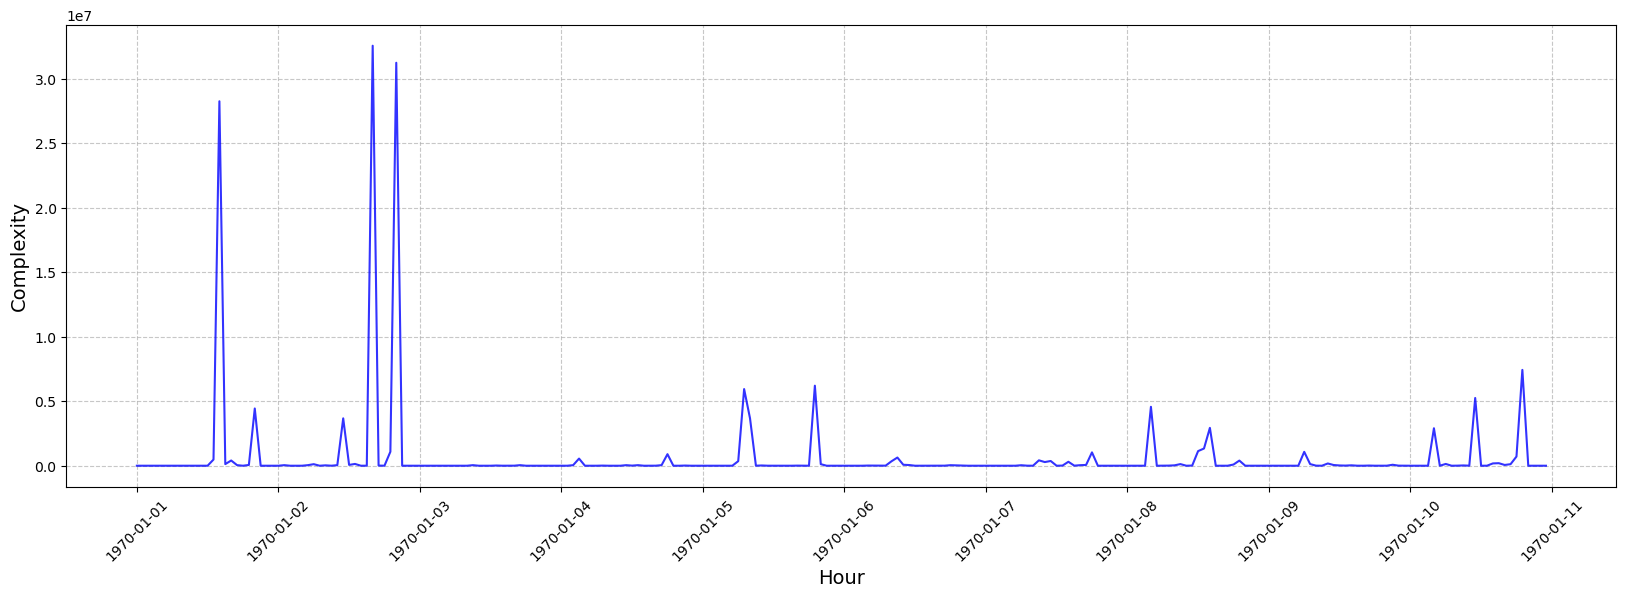
\includegraphics[width=0.8\linewidth]{img/hourly_complexity.png}
        \caption{Task complexity grouped by hour}
    \end{figure}
\end{frame}

\begin{frame}{Dataset Processing}
    \begin{figure}
        \centering
        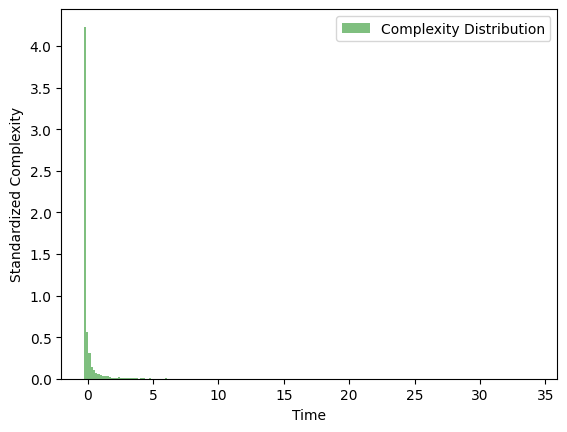
\includegraphics[width=0.7\linewidth]{img/task_complexity_distribution.png}
        \caption{High skewness of task complexity distribution}
    \end{figure}
\end{frame}


\printbibliography

\end{document}
